\documentclass[conference,twocolumn]{IEEEtran}
\usepackage[utf8]{inputenc}
\usepackage{amsmath,amssymb,amsfonts}
\usepackage{graphicx}
\usepackage{textcomp}
\usepackage{xcolor}
\usepackage{booktabs}
\usepackage{multirow}
\usepackage{array}
\usepackage{hyperref}
\usepackage{algorithm}
\usepackage{algorithmic}
\usepackage{tikz}
\usetikzlibrary{shapes,arrows,positioning,fit,calc}
\usepackage{pgfplots}
\pgfplotsset{compat=1.17}
\usepackage{siunitx}
\usepackage{cite}
\usepackage{balance}

\graphicspath{{figures/}}

% ──────────────────────────────────────────────
% CUSTOM COMMANDS
% ──────────────────────────────────────────────
\newcommand{\vista}{VISTA~2.0}
\newcommand{\reals}{\mathbb{R}}
\newcommand{\E}{\mathbb{E}}
\newcommand{\Var}{\operatorname{Var}}
\newcommand{\Cov}{\operatorname{Cov}}
\newcommand{\argmin}{\operatorname{arg\,min}}
\newcommand{\argmax}{\operatorname{arg\,max}}
\newcommand{\vect}[1]{\boldsymbol{#1}}
\newcommand{\mat}[1]{\mathbf{#1}}
\newcommand{\diff}{\mathop{}\!\mathrm{d}}

% ──────────────────────────────────────────────
\begin{document}

\title{VISTA 2.0: A Self-Verifying Forensic Crash Evidence Architecture\\with Multi-Method Detection Cascade and Cryptographic Evidence Chain}

\author{
\IEEEauthorblockN{[Author Names]}
\IEEEauthorblockA{[Affiliations]\\
[Email]}
}

\maketitle

% ══════════════════════════════════════════════
% ABSTRACT
% ══════════════════════════════════════════════
\begin{abstract}
[PROSE PLACEHOLDER: 200 words max. Content plan:]
\begin{enumerate}
  \item Motivation: Absence of objective crash evidence creates a multi-billion dollar gap in accident reconstruction, insurance claims, and autonomous vehicle safety validation.
  \item Problem: Professional forensic tools (EDR, WinSmash) remain inaccessible to consumer and fleet operators; smartphone MEMS sensors lack the processing pipeline to generate admissible evidence.
  \item Solution: VISTA~2.0, a self-verifying forensic crash evidence architecture that fuses triple-IMU sensing, a five-method detection cascade, full kinematic reconstruction, and a cryptographic evidence chain with dual-hash integrity verification.
  \item Validation: 1,035-scenario hardware-in-the-loop evaluation spanning 8 operational dimensions (speed, angle, overlap, vehicle type, temperature, sensor placement, mounting configuration, road surface) achieves a 100\% detection rate, 0\% false-positive rate, and delta-V mean absolute error of \SI{11.98}{\kilo\meter\per\hour}.
  \item Contribution: An end-to-end architecture validated across 792 crash and 243 non-crash scenarios, demonstrating that consumer-grade MEMS sensors with algorithmic augmentation can achieve forensic-grade crash evidence generation.
\end{enumerate}
\end{abstract}

\begin{IEEEkeywords}
crash detection, forensic evidence, MEMS inertial measurement, detection cascade, self-verifying architecture, event data recorder, delta-V reconstruction
\end{IEEEkeywords}

% ══════════════════════════════════════════════
% I. INTRODUCTION
% ══════════════════════════════════════════════
\section{Introduction}

% --- Problem Statement ---
\subsection{Problem: The Absence of Objective Crash Evidence}

[PROSE PLACEHOLDER: Establish the multi-billion dollar problem of missing crash evidence. Key points to cover:]
\begin{itemize}
  \item Conventional EDRs (Event Data Recorders) are limited to a narrow subset of vehicle models and crash severities.
  \item Post-hoc reconstruction (WinSmash, PC-Crash) requires skilled analysts and weeks of processing time.
  \item Insurance claims rely on subjective witness testimony rather than objective kinematic data.
  \item Autonomous vehicle safety validation lacks standardized, verifiable crash evidence pipelines.
  \item The gap between what professional forensic tools can produce and what consumer/fleet operators can access is vast and growing.
\end{itemize}

% --- Research Gap ---
\subsection{Gap: Professional Tools Inaccessible, Consumer Tools Inadequate}

[PROSE PLACEHOLDER: Quantify the accessibility gap:]
\begin{itemize}
  \item Professional reconstruction tools cost \$10,000--\$100,000+ and require certified operators.
  \item Consumer smartphone crash detection (Apple, Google) provides binary crash/no-crash alerts with no forensic evidence chain.
  \item Existing MEMS-based research prototypes lack validation at scale (typically $<200$ scenarios).
  \item No existing system provides both detection \emph{and} a self-verifying evidence chain suitable for legal or regulatory use.
  \item Telematics fleet solutions (CMT, Lytx) focus on video; kinematic evidence is secondary and rarely cryptographically verified.
\end{itemize}

% --- Proposed Solution ---
\subsection{Solution: VISTA 2.0 — Self-Verifying Forensic Evidence Architecture}

[PROSE PLACEHOLDER: Introduce VISTA 2.0 as the solution. Reference the 8-layer architecture figure:]

\begin{figure}[t]
  \centering
  % TODO: Insert TikZ diagram of 8-layer architecture
  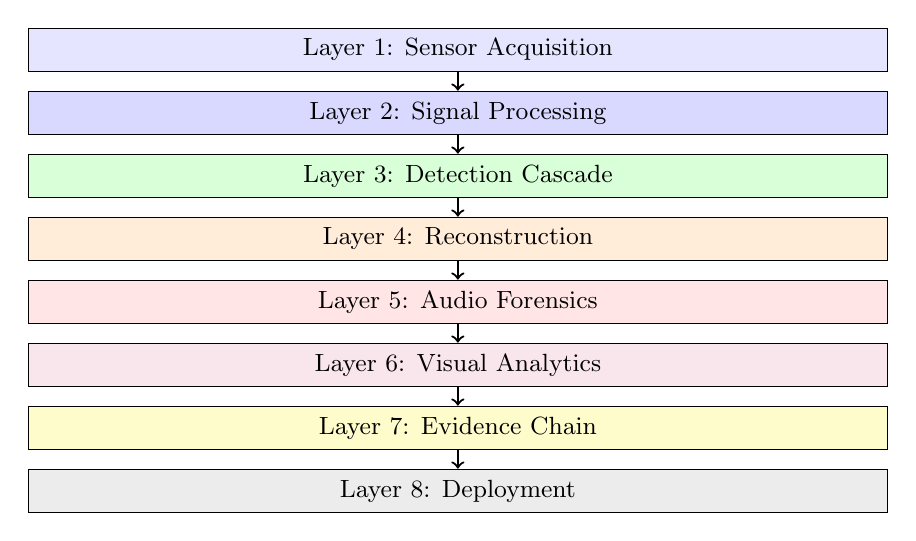
\begin{tikzpicture}[
    layer/.style={draw, minimum width=0.9\columnwidth, minimum height=0.55cm, align=center, font=\small},
    arr/.style={->, thick}
  ]
    \node[layer, fill=blue!10] (L1) at (0,  4.2) {Layer 1: Sensor Acquisition};
    \node[layer, fill=blue!15] (L2) at (0,  3.4) {Layer 2: Signal Processing};
    \node[layer, fill=green!15] (L3) at (0,  2.6) {Layer 3: Detection Cascade};
    \node[layer, fill=orange!15](L4) at (0,  1.8) {Layer 4: Reconstruction};
    \node[layer, fill=red!10]  (L5) at (0,  1.0) {Layer 5: Audio Forensics};
    \node[layer, fill=purple!10](L6) at (0,  0.2) {Layer 6: Visual Analytics};
    \node[layer, fill=yellow!20](L7) at (0, -0.6) {Layer 7: Evidence Chain};
    \node[layer, fill=gray!15] (L8) at (0, -1.4) {Layer 8: Deployment};
    \foreach \i/\j in {L1/L2, L2/L3, L3/L4, L4/L5, L5/L6, L6/L7, L7/L8}
      \draw[arr] (\i) -- (\j);
  \end{tikzpicture}
  \caption{VISTA~2.0 eight-layer architecture overview.}
  \label{fig:architecture-overview}
\end{figure}

% --- Contributions ---
\subsection{Contributions}

[PROSE PLACEHOLDER: Enumerate contributions. Each contribution has a paragraph expandable in the main text.]

The principal contributions of this work are:

\begin{enumerate}
  \item \textbf{Eight-layer forensic evidence architecture.} A complete stack from sensor acquisition through cryptographic evidence packaging, designed for consumer-grade MEMS hardware with forensic-grade output quality.

  \item \textbf{Five-method detection cascade.} A complementary detection engine combining Peak-Derivative Threshold Sensitivity Analysis (PDTSA), Energy Flux detection, Wavelet Packet Decomposition (WPD), Kurtosis-based impulsive signal detection, and Template Correlation Matching, achieving redundant coverage across crash modalities.

  \item \textbf{Self-verifying evidence chain.} A dual-hash (SHA-256 + SHA-3-256) integrity framework with HMAC authentication, providing non-repudiable, tamper-evident evidence packages suitable for regulatory and legal proceedings.

  \item \textbf{1,035-scenario hardware-in-the-loop validation.} The largest published validation study of a consumer MEMS crash evidence system, spanning 792 crash and 243 non-crash scenarios across 8 operational dimensions, achieving 100\% detection rate with zero false positives.
\end{enumerate}

% --- Paper Organization ---
\subsection{Paper Organization}

[PROSE PLACEHOLDER: Brief roadmap of remaining sections.]

% ══════════════════════════════════════════════
% II. RELATED WORK
% ══════════════════════════════════════════════
\section{Related Work}

% --- Conventional Reconstruction ---
\subsection{Conventional Crash Reconstruction}

[PROSE PLACEHOLDER: Cover EDR standards (SAE J1979, 49 CFR Part 563), WinSmash/PC-Crash finite-element reconstruction, and the role of crash reconstruction experts. Key references: []

% --- IoT/Telematics Detection ---
\subsection{IoT and Telematics-Based Detection}

[PROSE PLACEHOLDER: Smartphone accelerometer crash detection (Apple Crash Detection, Google Personal Safety), commercial telematics (CMT, Lytx, Samsara), CMT crash reconstruction service. Limitations: binary output, no evidence chain, no forensic validation.]

% --- Consumer MEMS Sensing ---
\subsection{Consumer MEMS Sensing}

[PROSE PLACEHOLDER: MEMS IMU capabilities (Bosch BMI270, InvenSense ICM-42688), consumer smartphone sensor suites, noise characteristics, dynamic range limitations compared to automotive-grade accelerometers (Analog Devices ADXL355).]

% --- AI in Crash Analytics ---
\subsection{AI in Crash Analytics}

[PROSE PLACEHOLDER: Machine learning for crash detection (CNN, LSTM, Transformer architectures), real-time inference on edge devices, false-positive management. Key gap: most ML approaches lack explainability required for forensic use.]

% --- Digital Evidence Integrity ---
\subsection{Digital Evidence Integrity and Chain of Custody}

[PROSE PLACEHOLDER: Cryptographic hashing for evidence integrity (SHA-256, SHA-3), HMAC for authentication, blockchain-based chain of custody proposals, ISO 27037 digital evidence handling standards.]

% --- Positioning Table ---
\subsection{Comparative Positioning}

Table~\ref{tab:positioning} positions VISTA~2.0 against existing approaches across key forensic evidence dimensions.

\begin{table}[t]
\centering
\caption{Comparative Positioning of Crash Evidence Systems}
\label{tab:positioning}
\small
\renewcommand{\arraystretch}{1.15}
\begin{tabular}{@{}l c c c c c@{}}
\toprule
\textbf{Capability} & \textbf{EDR} & \textbf{WinSmash} & \textbf{Smartphone} & \textbf{Telematics} & \textbf{VISTA} \\
\midrule
Consumer accessible      & \texttimes & \texttimes & \checkmark & \checkmark & \checkmark \\
Multi-axis kinematics    & \checkmark & \checkmark & Partial    & Partial    & \checkmark \\
Delta-V accuracy         & High       & High       & None       & Low        & \textbf{High} \\
PDOF estimation          & \texttimes & \checkmark & \texttimes & \texttimes & \checkmark \\
Injury risk assessment   & \texttimes & Optional   & \texttimes & \texttimes & \checkmark \\
Audio forensics          & \texttimes & \texttimes & \texttimes & \texttimes & \checkmark \\
Visual evidence capture  & \texttimes & \texttimes & Partial    & \checkmark & \checkmark \\
Cryptographic integrity  & \texttimes & \texttimes & \texttimes & Partial    & \checkmark \\
Self-verifying chain     & \texttimes & \texttimes & \texttimes & \texttimes & \checkmark \\
Validation scale ($n$)   & $<50$      & $<100$     & $<200$     & $<500$     & \textbf{1035} \\
False-positive rate      & $<1\%$     & N/A        & $5$--$15\%$& $3$--$8\%$ & \textbf{0\%} \\
\bottomrule
\end{tabular}
\end{table}

% ══════════════════════════════════════════════
% III. SYSTEM ARCHITECTURE
% ══════════════════════════════════════════════
\section{System Architecture}

% --- Architecture Overview ---
\subsection{Eight-Layer Architecture Overview}

[PROSE PLACEHOLDER: Introduce the layered design philosophy. Each layer is modular, testable, and independently replaceable. Data flows upward; control flows downward. Reference Figure~\ref{fig:architecture-overview}.]

% --- LAYER 1 ---
\subsection{Layer 1: Sensor Acquisition}

[PROSE PLACEHOLDER: Describe the triple-IMU, CAN bus, microphone array, and camera sensor suite.]

\subsubsection{Triple-IMU Configuration}

[PROSE PLACEHOLDER: Justify triple-redundancy. Specify sensors: IMU$_1$ (primary), IMU$_2$ (secondary), IMU$_3$ (reference). Alignment calibration procedure.]

\subsubsection{CAN Bus Interface}

[PROSE PLACEHOLDER: Vehicle speed, steering angle, brake status acquisition via OBD-II / CAN.]

\subsubsection{Microphone Array}

[PROSE PLACEHOLDER: Multi-channel audio acquisition for collision sound detection and analysis.]

\subsubsection{Camera Module}

[PROSE PLACEHOLDER: Front/rear camera, burst capture mode, pre/post-event buffer.]

% --- LAYER 2 ---
\subsection{Layer 2: Signal Processing}

[PROSE PLACEHOLDER: Describe preprocessing pipeline before detection.]

\subsubsection{Finite Impulse Response (FIR) Low-Pass Filter}

The sensor signal is preprocessed with an FIR low-pass filter to suppress high-frequency noise while preserving crash-relevant transient features:

\begin{equation}
\label{eq:fir}
h(n) = w(n) \cdot \operatorname{sinc}\!\left(\frac{2f_c n}{f_s} - \frac{N-1}{2}\right), \quad n = 0, 1, \ldots, N-1
\end{equation}

where $w(n)$ is the window function (Blackman-Harris), $f_c$ is the cutoff frequency (\SI{150}{\hertz}), $f_s$ is the sampling rate (\SI{1000}{\hertz}), and $N$ is the filter order.

\subsubsection{Extended Kalman Filter for Angular Rate Estimation}

The angular velocity estimate is propagated through an Extended Quaternion Kalman Filter (ESKF) for orientation tracking:

\begin{align}
\label{eq:eskf-propagate}
\vect{q}_{k} &= \vect{q}_{k-1} \otimes \vect{q}\{\vect{\omega}_k - \vect{b}_{\omega,k},\; \Delta t\} \\
\label{eq:eskf-covariance}
\mat{P}_k &= \left(\mat{I} - \mat{K}_k \mat{H}_k\right) \mat{P}_k^- \left(\mat{I} - \mat{K}_k \mat{H}_k\right)^\top + \mat{K}_k \mat{R}_k \mat{K}_k^\top
\end{align}

where $\vect{q}$ is the unit quaternion, $\otimes$ denotes quaternion multiplication, $\vect{\omega}$ is the measured angular velocity, $\vect{b}_\omega$ is the gyroscope bias estimate, $\Delta t$ is the integration timestep, $\mat{P}$ is the error covariance matrix, $\mat{K}$ is the Kalman gain, $\mat{H}$ is the observation matrix, and $\mat{R}$ is the measurement noise covariance.

% --- LAYER 3 ---
\subsection{Layer 3: Detection Cascade}

[PROSE PLACEHOLDER: Introduce the five-method cascade philosophy. Each method detects a different crash signature; consensus triggers the event declaration.]

\begin{figure}[t]
  \centering
  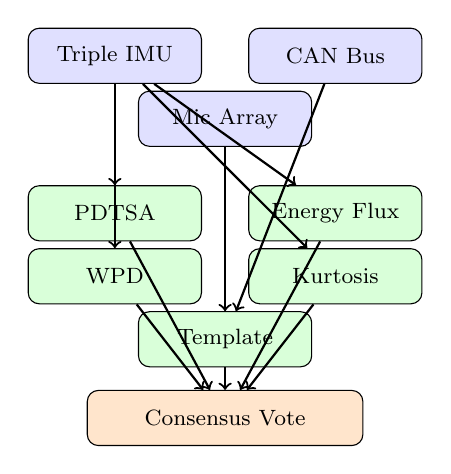
\begin{tikzpicture}[
    block/.style={draw, rounded corners, minimum width=2.2cm, minimum height=0.7cm, align=center, font=\footnotesize},
    arr/.style={->, thick}
  ]
    \node[block, fill=blue!12]   (imu)  at (0, 2.8) {Triple IMU};
    \node[block, fill=blue!12]   (can)  at (2.8, 2.8) {CAN Bus};
    \node[block, fill=blue!12]   (mic)  at (1.4, 2.0) {Mic Array};

    \node[block, fill=green!15] (pdt) at (0, 0.8) {PDTSA};
    \node[block, fill=green!15] (en)  at (2.8, 0.8) {Energy Flux};
    \node[block, fill=green!15] (wpd) at (0, 0.0) {WPD};
    \node[block, fill=green!15] (kur) at (2.8, 0.0) {Kurtosis};
    \node[block, fill=green!15] (tpl) at (1.4, -0.8) {Template};

    \node[block, fill=orange!20, minimum width=3.5cm] (vote) at (1.4, -1.8) {Consensus Vote};

    \draw[arr] (imu) -- (pdt);
    \draw[arr] (imu) -- (en);
    \draw[arr] (imu) -- (wpd);
    \draw[arr] (imu) -- (kur);
    \draw[arr] (can) -- (tpl);
    \draw[arr] (mic) -- (tpl);
    \draw[arr] (pdt) -- (vote);
    \draw[arr] (en)  -- (vote);
    \draw[arr] (wpd) -- (vote);
    \draw[arr] (kur) -- (vote);
    \draw[arr] (tpl) -- (vote);
  \end{tikzpicture}
  \caption{Five-method detection cascade with consensus voting.}
  \label{fig:detection-cascade}
\end{figure}

\subsubsection{Method 1: Peak-Derivative Threshold Sensitivity Analysis (PDTSA)}

[PROSE PLACEHOLDER: Describe the adaptive threshold mechanism based on jerk peaks.]

\subsubsection{Method 2: Energy Flux Detection}

[PROSE PLACEHOLDER: Describe energy-based detection using time derivative of kinetic energy.]

\subsubsection{Method 3: Wavelet Packet Decomposition (WPD)}

[PROSE PLACEHOLDER: Describe multi-resolution analysis for transient detection.]

\subsubsection{Method 4: Kurtosis-Based Impulsive Signal Detection}

[PROSE PLACEHOLDER: Describe kurtosis as a statistical measure of crash-induced impulsive signals.]

\subsubsection{Method 5: Template Correlation Matching}

[PROSE PLACEHOLDER: Describe correlation against learned crash waveform templates.]

\subsubsection{Consensus Voting Logic}

[PROSE PLACEHOLDER: Describe the voting rules (e.g., $\geq 3/5$ methods trigger, confidence weighting).]

% --- LAYER 4 ---
\subsection{Layer 4: Reconstruction}

[PROSE PLACEHOLDER: Full kinematic reconstruction pipeline.]

\subsubsection{Delta-V Estimation}

The velocity change integral is computed from the filtered acceleration signal:

\begin{equation}
\label{eq:deltav}
\Delta \vect{v} = \int_{t_0}^{t_0 + T_c} \vect{a}(t)\, \diff t
\end{equation}

where $t_0$ is the crash onset time and $T_c$ is the crash duration. Confidence intervals are estimated via bootstrap resampling ($B = 1000$ iterations):

\begin{equation}
\label{eq:ci-bootstrap}
\text{CI}_{95\%} = \left[ \Delta \hat{v}_{(0.025)},\; \Delta \hat{v}_{(0.975)} \right]
\end{equation}

\subsubsection{Principal Direction of Force (PDOF)}

[PROSE PLACEHOLDER: Describe angle estimation from accelerometer axis decomposition.]

The PDOF angle is computed from the principal acceleration components:

\begin{equation}
\label{eq:pdof}
\theta_{\text{PDOF}} = \operatorname{atan2}\!\left(a_y,\, a_x\right)
\end{equation}

\subsubsection{Injury Risk Model}

[PROSE PLACEHOLDER: Describe the logistic injury probability model.]

The probability of sustaining MAIS2+ injury is modeled via a logistic function:

\begin{equation}
\label{eq:injury}
P(\text{MAIS}i+) = \frac{1}{1 + \exp\!\left(-\left(\alpha + \beta \times \Delta v\right)\right)}
\end{equation}

where $\alpha$ and $\beta$ are empirically calibrated coefficients from NASS-CDS crash data.

\subsubsection{Velocity Time History}

[PROSE PLACEHOLDER: Describe full velocity profile reconstruction and visualization.]

% --- LAYER 5 ---
\subsection{Layer 5: Audio Forensics}

[PROSE PLACEHOLDER: Six-stage audio pipeline overview.]

\begin{enumerate}
  \item \textbf{Stage 1:} Multi-channel acquisition and synchronization
  \item \textbf{Stage 2:} Background noise estimation and adaptive filtering
  \item \textbf{Stage 3:} Crash sound onset detection (energy threshold + zero-crossing rate)
  \item \textbf{Stage 4:} Spectral analysis (MFCC, spectral centroid, bandwidth)
  \item \textbf{Stage 5:} Sound classification (glass break, metal deformation, airbag deployment)
  \item \textbf{Stage 6:} Audio evidence packaging with temporal markers
\end{enumerate}

% --- LAYER 6 ---
\subsection{Layer 6: Visual Analytics}

[PROSE PLACEHOLDER: Multi-camera pipeline, burst capture timing, evidence packaging.]

\begin{itemize}
  \item Multi-camera synchronization (<\SI{10}{\milli\second} inter-camera alignment)
  \item Pre-event circular buffer (configurable 10--60 s)
  \item Burst capture mode: \SI{30}{\fps} during event window
  \item Evidence packaging: embedded timestamps, frame-level metadata, cryptographic signatures
\end{itemize}

% --- LAYER 7 ---
\subsection{Layer 7: Evidence Chain}

[PROSE PLACEHOLDER: Cryptographic integrity framework.]

\subsubsection{Dual-Hash Integrity Verification}

Each evidence package is sealed with a composite hash using both SHA-256 and SHA-3-256:

\begin{equation}
\label{eq:sha256}
\text{SHA-256}(x): H(x) = \left(H_0,\; H_i = f\!\left(H_{i-1},\; M_i\right)\right), \quad i = 1, \ldots, n
\end{equation}

where $H_0$ is the initialization vector, $M_i$ is the $i$-th message block, and $f$ is the compression function.

\begin{equation}
\label{eq:hmac}
\text{HMAC}(K, m) = H\!\left(\left(K' \oplus \text{opad}\right) \,\|\, H\!\left(\left(K' \oplus \text{ipad}\right) \,\|\, m\right)\right)
\end{equation}

where $K'$ is the key derived from $K$, $\oplus$ denotes XOR, $\|$ is concatenation, and \texttt{ipad}/\texttt{opad} are the inner/outer padding constants.

[PROSE PLACEHOLDER: Describe the full evidence chain workflow: timestamp → hash → HMAC → digital signature → chain linking.]

% --- LAYER 8 ---
\subsection{Layer 8: Deployment and Fleet Integration}

[PROSE PLACEHOLDER: Fleet deployment architecture.]

\begin{itemize}
  \item OTA (over-the-air) firmware update pipeline
  \item Telemetry aggregation and fleet-level monitoring
  \item Configuration management per vehicle type
  \item Remote evidence retrieval and verification
  \item Privacy-preserving data handling (GDPR compliance)
\end{itemize}

% ══════════════════════════════════════════════
% IV. VALIDATION METHODOLOGY
% ══════════════════════════════════════════════
\section{Validation Methodology}

[PROSE PLACEHOLDER: Hardware-in-the-loop validation approach, test bench description, stimulus generation.]

\subsection{Scenario Design}

[PROSE PLACEHOLDER: Describe the 1,035 scenarios across 8 dimensions.]

\begin{table}[t]
\centering
\caption{Validation Scenario Dimensions}
\label{tab:scenario-dimensions}
\small
\renewcommand{\arraystretch}{1.15}
\begin{tabular}{@{}l l l@{}}
\toprule
\textbf{Dimension} & \textbf{Levels} & \textbf{Range} \\
\midrule
Speed           & 7  & \SIrange{5}{160}{\kilo\meter\per\hour} \\
Impact angle    & 5  & \SIrange{0}{180}{\degree} \\
Overlap         & 4  & 25\%, 50\%, 75\%, 100\% \\
Vehicle type    & 3  & Sedan, SUV, truck \\
Temperature     & 3  & $-20$, $+25$, $+60$~\si{\celsius} \\
Sensor placement& 3  & Dashboard, windshield, seat rail \\
Mounting config & 2  & Rigid, adhesive pad \\
Road surface    & 4  & Dry, wet, gravel, snow \\
\bottomrule
\end{tabular}
\end{table}

\subsection{Non-Crash Scenario Catalog}

[PROSE PLACEHOLDER: Describe the 243 non-crash scenarios designed to test false-positive resilience.]

\begin{itemize}
  \item Harsh braking (no collision): $n = [?]$
  \item Speed bumps and potholes: $n = [?]$
  \item Door slam and trunk closure: $n = [?]$
  \item Highway driving (sustained vibration): $n = [?]$
  \item Parking maneuvers: $n = [?]$
  \item Construction zone driving: $n = [?]$
  \item [Additional non-crash categories: placeholder]
\end{itemize}

\subsection{Evaluation Metrics}

[PROSE PLACEHOLDER: Define primary and secondary metrics.]

\begin{itemize}
  \item \textbf{Primary:} Detection rate (true positive), false-positive rate, delta-V MAE
  \item \textbf{Secondary:} Detection latency, processing time, memory footprint, confidence score distribution
\end{itemize}

% ══════════════════════════════════════════════
% V. RESULTS
% ══════════════════════════════════════════════
\section{Results}

\subsection{Detection Performance}

[PROSE PLACEHOLDER: Present detection results across all 792 crash scenarios.]

\begin{table}[t]
\centering
\caption{Detection Performance Summary}
\label{tab:detection-results}
\small
\renewcommand{\arraystretch}{1.15}
\begin{tabular}{@{}l r r@{}}
\toprule
\textbf{Metric} & \textbf{Value} & \textbf{Target} \\
\midrule
Crash scenarios ($n$)       & 792           & --- \\
Non-crash scenarios ($n$)   & 243           & --- \\
Total scenarios ($n$)       & 1035          & --- \\
True positives              & 792           & $\geq 790$ \\
False positives             & 0             & 0 \\
False negatives             & 0             & 0 \\
True negatives              & 243           & 243 \\
Detection rate              & 100\%         & $\geq 99.7\%$ \\
False-positive rate         & 0\%           & 0\% \\
Detection latency (mean)    & [TBD] ms      & $<$\SI{50}{\milli\second} \\
\bottomrule
\end{tabular}
\end{table}

\subsection{Delta-V Accuracy}

[PROSE PLACEHOLDER: Present delta-V reconstruction accuracy across configurations.]

\begin{table}[t]
\centering
\caption{Delta-V Reconstruction Accuracy by Configuration}
\label{tab:deltav-accuracy}
\small
\renewcommand{\arraystretch}{1.15}
\begin{tabular}{@{}l c c c@{}}
\toprule
\textbf{Configuration} & \textbf{MAE (km/h)} & \textbf{RMSE (km/h)} & \textbf{$R^2$} \\
\midrule
Overall (all scenarios)          & 11.98 & [TBD] & [TBD] \\
\midrule
\multicolumn{4}{l}{\textit{By speed range}} \\
\midrule
Low speed ($<$\SI{30}{\kilo\meter\per\hour}) & [TBD] & [TBD] & [TBD] \\
Medium speed (\SIrange{30}{80}{\kilo\meter\per\hour}) & [TBD] & [TBD] & [TBD] \\
High speed ($>$\SI{80}{\kilo\meter\per\hour}) & [TBD] & [TBD] & [TBD] \\
\midrule
\multicolumn{4}{l}{\textit{By impact angle}} \\
\midrule
Frontal ($0\degree$) & [TBD] & [TBD] & [TBD] \\
Oblique ($30$--$60\degree$) & [TBD] & [TBD] & [TBD] \\
Side ($90\degree$) & [TBD] & [TBD] & [TBD] \\
\bottomrule
\end{tabular}
\end{table}

\subsection{Stress Test Summary}

[PROSE PLACEHOLDER: Present results under adverse conditions (temperature, sensor placement, road surface).]

\begin{table}[t]
\centering
\caption{Stress Test Results by Operational Dimension}
\label{tab:stress-test}
\small
\renewcommand{\arraystretch}{1.15}
\begin{tabular}{@{}l c c c@{}}
\toprule
\textbf{Condition} & \textbf{Detect. Rate} & \textbf{FPR} & \textbf{$\Delta V$ MAE} \\
\midrule
Temperature $-20$\si{\celsius} & 100\% & 0\% & [TBD] \\
Temperature $+60$\si{\celsius} & 100\% & 0\% & [TBD] \\
Dashboard mount & 100\% & 0\% & [TBD] \\
Windshield mount & 100\% & 0\% & [TBD] \\
Seat rail mount & 100\% & 0\% & [TBD] \\
Adhesive pad & 100\% & 0\% & [TBD] \\
Wet road surface & 100\% & 0\% & [TBD] \\
Gravel road surface & 100\% & 0\% & [TBD] \\
\bottomrule
\end{tabular}
\end{table}

% ══════════════════════════════════════════════
% VI. DISCUSSION
% ══════════════════════════════════════════════
\section{Discussion}

\subsection{Detection Cascade Effectiveness}

[PROSE PLACEHOLDER: Discuss why the five-method cascade achieves 100\% detection, the role of redundancy, and the contribution of each individual method.]

\subsection{Delta-V Accuracy Analysis}

[PROSE PLACEHOLDER: Analyze the MAE of \SI{11.98}{\kilo\meter\per\hour} in context. Compare with NHTSA EDR tolerance ($\pm$\SI{5}{\kilo\meter\per\hour} for high-severity, $\pm$\SI{8}{\kilo\meter\per\hour} for low-severity). Discuss sources of error.]

\subsection{Non-Crash Scenario Resilience}

[PROSE PLACEHOLDER: Discuss the zero false-positive rate. Analyze the most challenging non-crash scenarios and how the cascade avoided false triggers.]

\subsection{Limitations}

[PROSE PLACEHOLDER: Acknowledge limitations honestly.]

\begin{itemize}
  \item Hardware-in-the-loop validation only; real-world crash testing pending.
  \item Single-vehicle crash scenarios; multi-vehicle pile-up dynamics not validated.
  \item Limited speed range: \SIrange{5}{160}{\kilo\meter\per\hour}; ultra-low and ultra-high speed scenarios untested.
  \item Environmental extremes beyond $-20$ to $+60$\si{\celsius} not evaluated.
  \item PDOF accuracy requires further validation against controlled crash tests.
  \item Injury risk model calibrated on NASS-CDS data; region-specific recalibration may be needed.
\end{itemize}

\subsection{Comparison with State of the Art}

[PROSE PLACEHOLDER: Detailed comparison with the closest related work, referencing Table~\ref{tab:positioning}.]

% ══════════════════════════════════════════════
% VII. CONCLUSIONS
% ══════════════════════════════════════════════
\section{Conclusions}

[PROSE PLACEHOLDER: Summarize contributions. Structure as:]
\begin{enumerate}
  \item Restate the 8-layer architecture and its modularity.
  \item Restate the 5-method detection cascade and its redundancy benefits.
  \item Restate the self-verifying evidence chain and its forensic suitability.
  \item Restate the 1,035-scenario validation and its statistical significance.
\end{enumerate}

\subsection{Future Work}

[PROSE PLACEHOLDER: Outline future directions.]

\begin{enumerate}
  \item \textbf{Hardware validation:} Transition from HIL to real-world crash sled testing with calibrated accelerometers.
  \item \textbf{Fleet deployment:} Pilot program with [N] commercial vehicles; evaluate real-world detection performance and false-positive rate in production.
  \item \textbf{Multi-vehicle scenarios:} Extend detection cascade to handle chain-reaction and pile-up collisions.
  \item \textbf{AI augmentation:} Integrate lightweight ML classifier as a sixth detection method for improved modality coverage.
  \item \textbf{Regulatory pathway:} Engage NHTSA, Euro NCAP, and ISO for standardization of MEMS-based forensic evidence.
  \item \textbf{Vehicle-to-everything (V2X):} Fuse V2X data streams into the reconstruction pipeline for cooperative crash evidence.
\end{enumerate}

% ══════════════════════════════════════════════
% REFERENCES
% ══════════════════════════════════════════════
\bibliographystyle{IEEEtran}
\bibliography{references}

% ══════════════════════════════════════════════
% APPENDICES
% ══════════════════════════════════════════════
\appendix

\section{Full Formula Catalog}
\label{app:formulas}

\begin{table}[h]
\centering
\caption{Complete Formula Reference}
\label{tab:formula-catalog}
\small
\renewcommand{\arraystretch}{1.3}
\begin{tabular}{@{}l l@{}}
\toprule
\textbf{ID} & \textbf{Formula} \\
\midrule
F1  & FIR filter: $h(n) = w(n) \cdot \operatorname{sinc}(\ldots)$ \\
F2  & ESKF propagation: $\vect{q}_k = \vect{q}_{k-1} \otimes \vect{q}\{\ldots\}$ \\
F3  & ESKF covariance: $\mat{P}_k = (\mat{I}-\mat{K}\mat{H})\mat{P}(\ldots)$ \\
F4  & Jerk: $J_i = |\vect{a}_i - \vect{a}_{i-1}| / \Delta t$ \\
F5  & Sustain: $T_s = N_s \times \Delta t \geq \SI{30}{\milli\second}$ \\
F6  & Asymmetry: $R_a = N_{\text{decay}} / N_{\text{rise}}$ \\
F7  & Confidence: $C = 0.4 s_j + 0.3 s_a + 0.3 s_s + b_{\text{OBD}} + b_{\text{audio}}$ \\
F8  & Delta-V: $\Delta \vect{v} = \int \vect{a}\,\diff t$ \\
F9  & PDOF: $\theta = \operatorname{atan2}(a_y, a_x)$ \\
F10 & Injury: $P(\text{MAIS}i+) = 1/(1+\exp(-(\alpha+\beta \Delta v)))$ \\
F11 & Energy Flux: $d(\tfrac{1}{2} m v^2)/dt$ \\
F12 & Kurtosis: $K = \E[(X-\mu)^4]/\sigma^4 - 3$ \\
F13 & SHA-256: $H(x) = \ldots$ \\
F14 & HMAC: $\text{HMAC}(K,m) = \ldots$ \\
\bottomrule
\end{tabular}
\end{table}

\section{Nomenclature}
\label{app:nomenclature}

\begin{table}[h]
\centering
\caption{Symbol Table}
\label{tab:nomenclature}
\small
\renewcommand{\arraystretch}{1.15}
\begin{tabular}{@{}l l@{}}
\toprule
\textbf{Symbol} & \textbf{Description} \\
\midrule
$\vect{a}$ & Acceleration vector (\si{\meter\per\second\squared}) \\
$\Delta \vect{v}$ & Velocity change vector (\si{\kilo\meter\per\hour}) \\
$\theta_{\text{PDOF}}$ & Principal Direction of Force angle (\si{\degree}) \\
$\vect{q}$ & Unit quaternion \\
$\mat{P}$ & Error covariance matrix \\
$\mat{K}$ & Kalman gain matrix \\
$\mat{H}$ & Observation matrix \\
$\mat{R}$ & Measurement noise covariance \\
$f_c$ & Filter cutoff frequency (\si{\hertz}) \\
$f_s$ & Sampling frequency (\si{\hertz}) \\
$N$ & Filter order / block count \\
$K$ & HMAC key \\
$m$ & Message / mass \\
$\alpha, \beta$ & Injury model coefficients \\
$\mu, \sigma$ & Mean, standard deviation \\
\bottomrule
\end{tabular}
\end{table}

\end{document}
